\documentclass{article}
\usepackage{ja}
\usepackage{epsfig} %(this is to import figures)
\usepackage{graphicx}
\usepackage[spanish,activeacute]{babel} 
\usepackage[backend=biber,style=numeric,sorting=none]{biblatex}
\addbibresource{referencias.bib}
\usepackage{amsmath}
\usepackage{float}
\usepackage{tikz}          % para dibujar con TikZ
\usepackage{graphicx}      % para incluir imágenes
\usepackage{eso-pic}       % (opcional) útil si usas overlay sobre la página
\addto\captionsspanish{\renewcommand{\tablename}{Tabla}}
\usepackage{listings}   % <-- este es el paquete necesario
\usepackage{xcolor}     % <-- opcional, pero recomendado para colores
\usepackage{listings}
\usepackage{xcolor}
\usepackage[hidelinks]{hyperref}
\lstset{
  language=Python,
  basicstyle=\ttfamily\footnotesize,     % tipo y tamaño de fuente
  backgroundcolor=\color{gray!10},       % <-- fondo gris claro
  frame=single,                          % borde alrededor del código
  numbers=left,                          % numeración de líneas a la izquierda
  numberstyle=\tiny\color{gray},         % estilo de los números
  keywordstyle=\color{blue},             % color de palabras clave
  stringstyle=\color{orange!90!black},   % color de strings
  commentstyle=\color{green!50!black},   % color de comentarios
  showstringspaces=false,
  breaklines=true,                       % partir líneas largas
  breakatwhitespace=true,
  columns=fullflexible
}


\title{\huge Midiento experimentalmente la aceleración de gravedad y
la constante elastica de un resorte}

\author{Ignacio Villagrán Melgarejo}

\begin{document}

\maketitle

\begin{tikzpicture}[remember picture, overlay]
    \node[anchor=north west, xshift=2.6cm, yshift=-0.5cm] at (current page.north west)
    {
\includegraphics[width=3.5cm]{img/marcaderecha.png}};
    \node[anchor=north east, xshift=-2.6cm, yshift=-1cm] at (current page.north east)
    {
\includegraphics[width=4cm]{img/logo-cfm.png}};
\end{tikzpicture}

\begin{abstract}
{\em El presente informe tiene como objetivo mostrar los resultados de dos
experimentos. En el primero medimos la 
aceleración de gravedad ``$g$'' utilizando un modelo que consiste en un cuerpo
que cae con cierta inclinación y mediremos el tiempo que tarda en recorrer
una distancia determinada. En el segundo experimento, medimos la constante
elastica de un resorte usando el valor de g obtenido en el experimento
anterior. A partir de los datos obtenidos, aplicaremos las leyes de
movimiento, la Ley de Hooke y la segunda Ley de Newton, ademas de codigos en
Python, para facilitar y automatizar el proceso de cálculo.} \\

{\bf Palabras clave:} aceleración de gravedad, constante elástica, segunda 
Ley de Newton, Ley de Hooke, resorte, Python.\\
\end{abstract}

\section*{Introducción}
¿Que es la aceleración de gravedad? Para responder esta pregunta,
debemos primero definir que es la gravedad. La gravedad es una fuerza
de atracción que existe entre dos cuerpos con masa. Esta fuerza es
responsable de que los objetos caigan hacia la Tierra cuando se sueltan.
La aceleración de gravedad, denotada comúnmente como $g$, se define como
el incremento constante de la velocidad por unidad de tiempo percibido
por un cuerpo en caida libre, es directamente proporcional a la fuerza $F$
en newtons (N) e inversamente proporcional a la masa $m$ del cuerpo en
kilogramos (kg) \cite{metas2002}. Matematicamente, se expresa:

\begin{equation}
g = \frac{F}{m}
\end{equation}

Nosotros vamos a medir la aceleración de gravedad utilizando un método
experimental basado en la caída libre de objetos. Para ello, trabajaremos
con un modelo que consiste en un cuerpo que cae con cierta inclinación y
mediremos el tiempo que tarda en recorrer una distancia determinada
variando el angulo de inclinación. A partir de los datos obtenidos, 
aplicaremos la segunda Ley de Newton y leyes de movimiento uniformemente
acelerado para obtener un modelo que relacione el tiempo de caida con el
angulo de inclinación, de esta forma haremos un ajuste de recta a los datos
usando progamas en python para asi obtener finalmente un valor para la
aceleración de gravedad. Una vez que tengamos $g$, pasaremos al segundo 
experimento en el que mediremos la constante elastica $k$ de un resorte.
¿Como lo haremos? Mediremos la deformación que sufre el resorte al colgar
sobre el distintas masas. Con las 
mediciones obtenidas y haciendo uso de la Ley de Hooke y la segunda Ley de 
Newton, obtendremos una expresión que relacione nuestras variables. 
Finalmente haremos un promedio de los valores obtenidos de $k$ teniendo 
cuidado con ciertos valores atípicos que puedan afectar el resultado.

\section*{Marco teorico}
Segunda Ley de Newton: La segunda ley de Newton o principio fundamental 
establece que las aceleraciones que experimenta un cuerpo son proporcionales 
a las fuerzas que recibe. Matematicamente se escribe como:
\begin{equation}
F = m a
\end{equation}
donde $F$ es la fuerza neta aplicada al objeto, $m$ es la masa del objeto
y $a$ es la aceleración del objeto \cite{fisicalab2025principio}. \\

Ley de Hooke: Establece que, dentro de ciertos límites, la fuerza requerida 
para estirar un objeto elástico, como un resorte de metal, es directamente 
proporcional a la extensión del resorte. Comúnmente la escribimos así:
\begin{equation}
F = -k x
\end{equation}
donde $F$ es la fuerza aplicada al resorte, $k$ es la constante de resorte
y $x$ es la distancia que el resorte se estira o comprime desde su
posición de equilibrio \cite{khan2019hooke}. \\

Ecuación general de movimiento rectilíneo uniformemente acelerado (MRUA):
El MRUA es un tipo de movimiento en el cual un objeto se desplaza en línea
recta con una aceleración constante. La ecuación que describe este tipo de
movimiento es:
\begin{equation}
d = v_i t + \dfrac{1}{2} a t^2
\end{equation}
donde $d$ es la distancia recorrida por el objeto, $v_i$ es la velocidad
inicial del objeto, $a$ es la aceleración constante y $t$ es el tiempo.
Como veremos mas adelante nuestro objeto a estudio parte del reposo, osea
que la velocidad inicial es cero asi que nuestra expresion queda reducida a:
\begin{equation}
d = \dfrac{1}{2} a t^2
\end{equation}

Aceleración de un objeto que se desliza por un plano inclinado de ángulo 
($\theta$) respecto a la horizontal, sin fricción:
\begin{equation}
a = g \sin(\theta)
\end{equation}
donde $g$ es la aceleración de gravedad y $\theta$ es el ángulo de inclinación
del plano \cite{serway2014physics}.

\section*{Procedimiento experimental}
Partiremos armando el experimento, bastante simple por cierto. Tenemos
un barra inclinada con cierto angulo que cambiaremos segun queramos y 
un movil que haremos caer desde el punto mas alto de la barra. Mediremos
el tiempo que tarda en caer con un cronometro, tomaremos 5 medidas de tiempo
por cada angulo de inclinación. Nosotros tomamos medidas para 13 angulos. 
Luego que tengamos todas las mediciones tomaremos el promedio de tiempo 
para cada angulo, usando un programa en python automatizamos esta tarea.
En la siguiente tabla mostramos estos promedios:

\begin{table}[H]
\centering
\begin{tabular}{|c|c|c|c|}
\hline
$\theta$ (°) & $\bar{t}$ $\pm$ 0.005 (s) & $\theta$ (°) & $\bar{t}$ $\pm$ 0.005 (s) \\
\hline
1 & 8.70 & 8 & 0.97 \\
\hline
2 & 2.97 & 9 & 0.94 \\
\hline
3 & 2.34 & 10 & 1.05 \\
\hline
4 & 1.90 & 11 & 0.80 \\
\hline
5 & 1.58 & 14 & 0.82 \\
\hline
6 & 1.25 & 20 & 0.79 \\
\hline
7 & 1.10 & & \\
\hline
\end{tabular}
\caption{Promedios de los tiempos}
\label{tab:promedios-tiempos}
\end{table}

Si graficamos tanto los datos crudos como los promedios obtenemos el 
siguiente grafico donde los puntos rojos representan los promedios de 
los datos:
\begin{figure}[H]
\centering
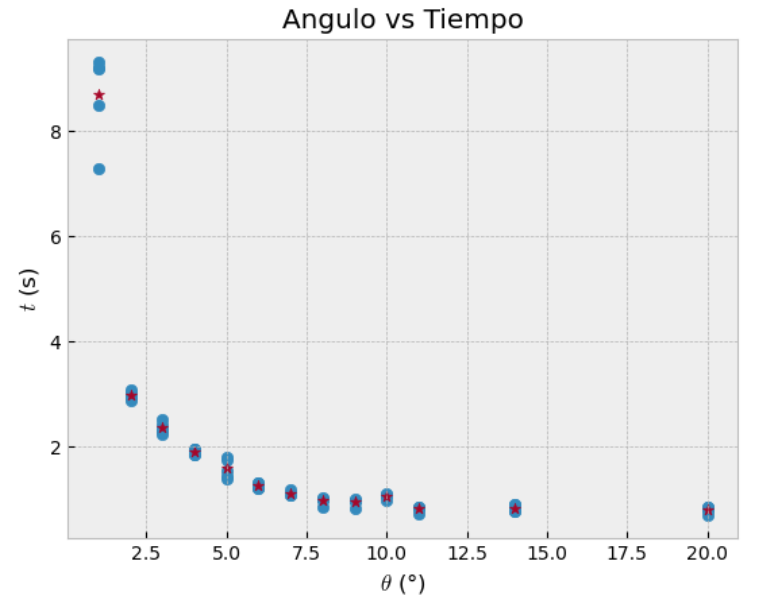
\includegraphics[scale=0.55]{img/grafico1.png}
\caption{Ángulo vs tiempo}
\label{fig:angulo-tiempo}
\end{figure}

Ahora quisieramos hacer un ajuste lineal, para ello despejamos $t$ en la 
ecuación (5), reemplazamos $a = g \sin(\theta)$ y consideramos $d = 0.95$ 
m, debemos llegar a la siguiente expresión:
\begin{equation}
   t = \sqrt{\dfrac{2d}{g}} \dfrac{1}{\sqrt{\sin(\theta)}}
\end{equation}

Inmediatamente notamos que el modelo no es lineal asi que para linealizarlo definimos 
$x = 1/\sqrt{\sin(\theta)}$, de esta manera nuestro modelo queda como 
$t = m x$, con $m = \sqrt{2d/g}$. Cabe mencionar que descartamos el ultimo
dato ya que este se aleja mucho de los demas. Procedemos a graficar $x$ vs 
$t$ con sus respectivas barras de error:
\begin{figure}[H]
\centering
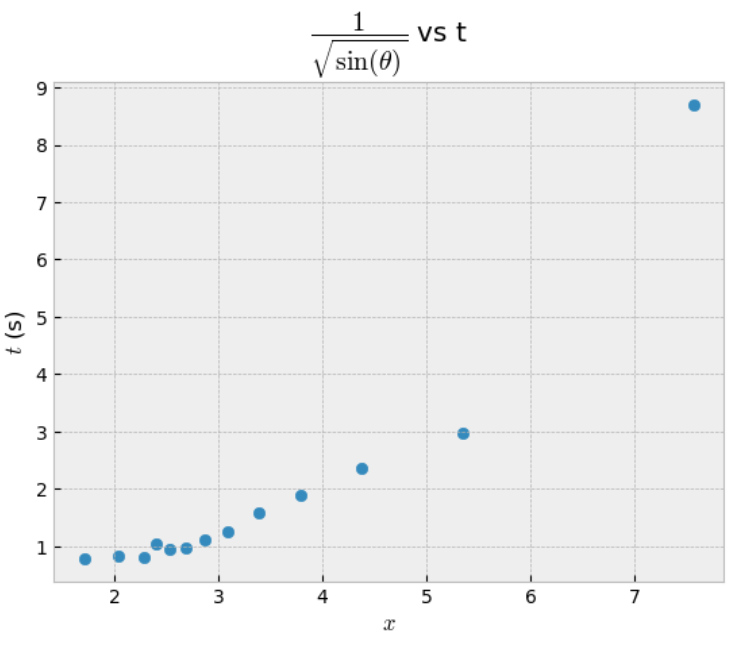
\includegraphics[scale=0.55]{img/grafico2.png}
\caption{Gráfico $\dfrac{1}{\sqrt{\sin(\theta)}}$ vs tiempo}
\label{fig:ajuste-lineal}
\end{figure}

Haciendo un ajuste lineal en python con polyfit obtenemos que la pendiente 
de la recta que mas se ajusta al modelo es $m = 0.516$. No graficamos la
recta ya que solo nos interesa el valor de la pendiente. Luego usando la 
ecuación (7) y sabiendo que $\sqrt{\frac{2d}{g}} = m$ podemos despejar $g$:
\begin{equation}
   g = \dfrac{2d}{m^2}
\end{equation}

Que nos da un valor de $g = 7.18 \, \text{m/s}^2$. \\

Para estimar el error en $g$, tenemos que 
\begin{equation}
   g = g(t,\theta) = \dfrac{2d}{t} \dfrac{1}{\sin(\theta)}
\end{equation}

Entonces $\delta g$ está dado por:
\begin{equation}
   \delta g = \left| \dfrac{\partial g}{\partial t} 
   \right| \Delta t + \left| \dfrac{\partial g}{\partial \theta} \right| 
   \Delta \theta
\end{equation}

Calculando las derivadas parciales tenemos:
\begin{equation}
   \dfrac{\partial g}{\partial t} = -\dfrac{2d}{t^2 \sin(\theta)}
\end{equation}
y
\begin{equation}
   \dfrac{\partial g}{\partial \theta} = -\dfrac{2d \cos(\theta)}{t \sin^2(\theta)}
\end{equation}

Considerando que $\Delta t$ nos da 0.3 s y $\Delta \theta$ nos da 0.6 rad,
evaluamos $t$ y $\theta$ con sus respectivos promedios $\bar{t} = 1.93$ s y
$\bar{\theta} = 0.13$ rad, obteniendo $\delta g = 5.5 \, \text{m/s}^2$. \\

Finalmente reportamos el valor de la aceleración de gravedad como: 
$g = 7.2 \, \pm 5.5 \; \text{m/s}^2$. \\

Para la siguiente parte del experimento, como ya obtuvimos el valor de $g$, 
mediremos la constante elastica de un resorte. Para ello, colgaremos 
diferentes masas al resorte y mediremos la deformación que sufre el resorte
debido a la fuerza que ejerce la gravedad. \\

Por segunda Ley de Newton, 
tenemos que:
\begin{equation}
   \sum F = ma
\end{equation}
Considerando que la fuerza neta es la fuerza del resorte (Ley de Hooke) 
menos la fuerza de gravedad, y que el resorte está en equilibrio tenemos:
\begin{equation}
   kx - mg = 0
\end{equation}
De donde podemos despejar la constante elastica $k$:
\begin{equation}
   k = \dfrac{mg}{x}
\end{equation}
donde $m$ es la masa colgada del resorte, $g$ es la aceleración de gravedad
y $x$ es la deformación del resorte. \\

Se tomaron un total de 14 mediciones con diferentes masas y se midió la
deformación del resorte en cada caso, asi como la constante elastica usando
la ecuación (11). A continuación se muestra una tabla con los datos 
obtenidos:

\begin{table}[H]
\centering
\begin{tabular}{|c|c|c|}
\hline
Masa (kg) & Deformación (m) & k (N/m) \\
\hline
0.2500 & 0.075 & 23.93 \\
\hline
0.4997 & 0.154 & 23.29 \\
\hline
0.9996 & 0.311 & 23.07 \\
\hline
0.0477 & 0.009 & 38.05 \\
\hline
0.0258 & 0.003 & 61.74 \\
\hline
0.7975 & 0.249 & 22.99 \\
\hline
0.3399 & 0.102 & 23.92 \\
\hline
0.0406 & 0.004 & 72.87 \\
\hline
1.1228 & 0.355 & 22.70 \\
\hline
0.1872 & 0.053 & 25.36 \\
\hline
0.0900 & 0.023 & 28.09 \\
\hline
0.1054 & 0.030 & 25.22 \\
\hline
0.7497 & 0.236 & 22.80 \\
\hline
0.4168 & 0.128 & 23.37 \\
\hline
\end{tabular}
\caption{Mediciones de masa, deformación y constante elástica}
\label{tab:mediciones-resorte}
\end{table}

Si nos damos cuenta, hay unos valores que se disparan, estos son los
valores correspondientes a masas muy pequeñas, lo que genera una gran
incertidumbre en la medición de la deformación del resorte. Por lo tanto,
decidimos eliminar estos valores atípicos y quedarnos solo con los valores
más confiables. \\

Usamos un codigo en python para calcular el promedio de las constantes 
elasticas obtenidas, resultando en un valor de $k = 31.24 \, \text{N/m}$
tomando todos los valores y $k = 24.07 \, \text{N/m}$ si solo consideramos
los valores confiables. Con respecto al error del promedio este está dado
por:
\begin{equation}
   \delta k = \dfrac{\sigma}{\sqrt{n}}
\end{equation}
donde $\sigma$ es la desviación estándar de los valores de $k$ obtenidos
y $n$ es el número de mediciones. Calculando esto obtenemos un error de
$0.462 \, \text{N/m}$. \\

Finalmente reportamos $k = 24.1 \, \pm 0.5 \; \text{N/m}$. \\

\section*{Resultados}
Obtuvimos un valor de $g = 7.2 \, \text{m/s}^2$ con un error de $5.5$ m/s$^2$
para la constante de gravedad y un valor de $k = 24.1 \,
\text{N/m}$ con un error de $0.5 \, \text{N/m}$ para la constante elástica 
del resorte.

\section*{Discusión}
Con respecto al valor de $g$, este se encuentra algo alejado del 
valor aceptado de $9.81 \,\text{m/s}^2$ y teniendo en cuenta el error asociado,
este oscila entre $1.7 \,\text{m/s}^2$ y $12.7 \,\text{m/s}^2$. Lo más probable
es que esto se deba a errores sistemáticos en la medición
de tiempo, ya que usamos un cronómetro manual, lo que introduce un error
humano. También asumimos condiciones ideales, como la ausencia de fricción,
lo que pudo haber afectado el resultado. \\

En cuanto al valor de $k$, este se encuentra dentro de un rango aceptable,
considerando que los valores atípicos fueron eliminados. Sin embargo,
es importante destacar que la precisión del valor de $k$ depende en gran
medida del valor de $g$ utilizado en los cálculos, asi que es importante 
mencionar que cualquier error en la medición de $g$ se reflejará en el valor 
de $k$.
 

\section*{Conclusiones}
Considerando que el experimento se realizó con herramientas básicas y
que se asumieron condiciones ideales, los resultados obtenidos son
razonables. Para mejorar la precisión, se podrían implementar
métodos de medición mejores y controles experimentales más rigurosos.
Sin embargo, los resultados obtenidos proporcionan una buena aproximación
a los valores reales de $g$ y $k$, demostrando que los principios 
de la fisica pueden ser aplicados con éxito incluso en condiciones 
de no tanto profesionalismo.

Esta experiencia nos permitió comprender mejor las principales leyes 
de la mecanica, específicamente la segunda Ley de Newton y la Ley de Hooke.
Obligandonos a mezclar distintos modelos y conceptos con el fin de cumplir
nuestros objetivos.
Además, pudimos enriquecer nuestras habilidades en programación, ya que
constantemente usamos programas en Python para analizar los datos obtenidos
durante el experimento o simplemente para automatizar tareas. En resumen, 
todos los laboratorios que realizamos en lo que va del curso han sido de 
gran utilidad para nuestro aprendizaje y desarrollo como futuros 
profesionales.
\vspace{1.3cm}

\section*{Codigos utilizados}

\begin{lstlisting}[language=Python, caption= Código para importar librerias 
   y datos]
import numpy as np
import matplotlib.pyplot as plt
plt.style.use("bmh")
datos = np.genfromtxt("datos_crudos_movil.txt")
\end{lstlisting}


\begin{lstlisting}[language=Python, caption= Código para calcular promedios de tiempos]
theta = datos[:,0]
tiempo = datos[:,1]

promedios = []
for i in range(0, len(valores), 5):
    bloque = valores[i:i+5]
    prom = np.mean(bloque)
    promedios.append(prom)
promedios = np.array(promedios)

thetas = np.unique(theta) 

\end{lstlisting}

\begin{lstlisting}[language=Python, caption= Código para graficar datos y 
   promedios]
plt.scatter(theta,tiempo)
plt.grid(True)
plt.scatter(thetas,promedios,marker = "*")
plt.title("Angulo vs Tiempo")
plt.xlabel("$\theta$ (grados)")
plt.ylabel("$t$ (s)")
plt.show()
\end{lstlisting}

\begin{lstlisting}[language=Python, caption= Código para pasar 
   ángulos a radianes y linealizar modelo]
theta_radianes = thetas * np.pi / 180
x = 1 / np.sqrt(np.sin(theta_radianes))
\end{lstlisting}

\begin{lstlisting}[language=Python, caption= Código para graficar 
   modelo linealizado]
plt.errorbar(x[1:13], promedios[1:13],yerr=Dt[1:13], fmt="o")
plt.xlabel("$x$")
plt.ylabel("$t$ (s)")
plt.title("$\dfrac{1}{\sqrt{\sin(\\theta)}}$ vs t")
plt.show()
\end{lstlisting}

\begin{lstlisting}[language=Python, caption= Código para el ajuste lineal]
coef = np.polyfit(x,promedios,1)
m, b = coef
\end{lstlisting}

\begin{lstlisting}[language=Python, caption= Código para calcular $k$]
g = 7.18

def constante_elastica(m,x):
    return(m*g / x)

k = constante_elastica(m_kilos,x_metros)

print(np.mean(k))

k_reales = k[[0,1,2,5,6,8,9,10,11,12,13]]
print(np.mean(k_reales))
\end{lstlisting}


\newpage
\printbibliography


%Copyright (no borrar)

\vspace{1cm}
\setbox0\vbox{\noindent

\includegraphics[width=0.18\textwidth]{logo-cc-by-nc-sa}}
\wd0=0pt\ht0=0pt\box0
\hangindent=33mm\hangafter =-3\vspace{-4mm} 
\small
\copyright{}{\@ \the\year} by the authors. Submitted for possible open access publication under the terms and conditions of the Creative Commons Attribution CC BY-NC-SA 4.0 license (https://creativecommons.org/licenses/by-nc-sa/4.0/deed.es).

\end{document}
